\def\year{2015}
\documentclass[letterpaper]{article}

\usepackage{aaai}
\usepackage{times}
\usepackage{helvet}
\usepackage{courier}

\usepackage{graphicx}
\usepackage{amsmath}
\usepackage{amssymb}
\usepackage{amsthm}

\usepackage{algorithm}
\usepackage{algpseudocode}

\frenchspacing
\setlength{\pdfpagewidth}{8.5in}
\setlength{\pdfpageheight}{11in}

\pdfinfo{
/Title (Insert Your Title Here)
/Author (Put All Your Authors Here, Separated by Commas)}

\setcounter{secnumdepth}{0}  

% We define our own macros here
\newcommand{\mat}[1]{\mathbf{#1}}
\newcommand{\A}{\mat{A}}
\newcommand{\B}{\mat{B}}
\newcommand{\M}{\mat{M}}
\renewcommand{\H}{\mat{H}}
\newcommand{\Rset}{\mathbb{R}}
\newcommand{\R}{\Rset}
\newcommand{\Nset}{\mathbb{N}}
\newcommand{\Hset}{\mathbb{H}}
\newcommand{\sstar}{\Sigma^\star}
\newcommand{\Sstar}{\sstar}

\newcommand{\pivec}{\boldsymbol{\pi}}
\newcommand{\alphavec}{\boldsymbol{\alpha}}
\newcommand{\thetavec}{\boldsymbol{\theta}}
\newcommand{\rhovec}{\boldsymbol{\rho}}
\newcommand{\vecalpha}{\alphavec}
\newcommand{\vectheta}{\thetavec}
\newcommand{\vecrho}{\rhovec}
\newcommand{\aone}{\boldsymbol{\alpha}_\epsilon}
%\newcommand{\aone}{\boldsymbol{\alpha}_0}
\newcommand{\ainf}{\boldsymbol{\alpha}_{\infty}}
\newcommand{\taone}{\tilde{\boldsymbol{\alpha}}_0}
\newcommand{\tainf}{\tilde{\boldsymbol{\alpha}}_{\infty}}
\newcommand{\haone}{\hat{\boldsymbol{\alpha}}_0}
\newcommand{\hainf}{\hat{\boldsymbol{\alpha}}_{\infty}}
\newcommand{\bone}{\boldsymbol{\beta}_0}
\newcommand{\binf}{\boldsymbol{\beta}_{\infty}}
\newcommand{\vecb}{\boldsymbol{\beta}}
\newcommand{\tbone}{\tilde{\boldsymbol{\beta}}_0}
\newcommand{\tbinf}{\tilde{\boldsymbol{\beta}}_{\infty}}
\newcommand{\hbone}{\hat{\boldsymbol{\beta}}_0}
\newcommand{\hbinf}{\hat{\boldsymbol{\beta}}_{\infty}}
\newcommand{\Alpha}{\aone}
\newcommand{\Beta}{\ainf}
\newcommand{\psrA}{\mathcal{A}}
\newcommand{\psr}{\langle  \aone, \ainf, \{\A_\sigma\} \rangle}
\newcommand{\psrsigma}{\langle \Sigma, \aone, \ainf, \{\A_\sigma\}_{\sigma \in \Sigma} \rangle}
\newcommand{\mpsrsigma}{\langle \Sigma, \Sigma', \kappa, \aone, \ainf, \{\A_\sigma\}_{\sigma \in \Sigma'} \rangle}

%\newcommand{\wb}{\langle  \bone, \binf, \{\B_\sigma\} \rangle}
%\newcommand{\wap}{\langle  \aone', \ainf', \{\A'_\sigma\} \rangle}
%\newcommand{\wbp}{\langle  \bone', \binf', \{\B'_\sigma\} \rangle}
%\newcommand{\wat}{\langle  \taone, \tainf, \{\tilde{\A}_\sigma\} \rangle}
%\newcommand{\wtt}{\langle  \taone, \tainf, \{\tilde{\A}_\sigma^\delta\} \rangle}
%\newcommand{\wt}{\langle  \aone, \ainf, \{{\A}_\sigma^\delta\} \rangle}
%\newcommand{\wbt}{\langle  \tbone, \tbinf, \{\tilde{\B}_\sigma\} \rangle}
%\newcommand{\wah}{\langle  \haone, \hainf, \{\hat{\A}_\sigma\} \rangle}
%\newcommand{\wbh}{\langle  \hbone, \hbinf, \{\hat{\B}_\sigma\} \rangle}

\newcommand{\Bs}{\mathcal{B}}
\newcommand{\cB}{\Bs}
\newcommand{\Ps}{\mathcal{P}}
\newcommand{\Ss}{\mathcal{S}}
\newcommand{\cW}{\mathcal{W}}
\newcommand{\Vsv}{\mat{V}}

\DeclareMathOperator*{\argmax}{\rm argmax}
\DeclareMathOperator*{\argmin}{\rm argmin}
\DeclareMathOperator{\sgn}{sgn}
\DeclareMathOperator{\sign}{sign}
\DeclareMathOperator{\range}{range}
\DeclareMathOperator{\rank}{rank}
\DeclareMathOperator{\diag}{diag}
\DeclareMathOperator{\local}{local}
\DeclareMathOperator{\Tr}{Tr}

\usepackage[textsize=footnotesize,color=green!40]{todonotes}
\newcommand{\borja}[1]{\todo[inline,color=green!40]{{\it Borja:~}#1}}
\newcommand{\doina}[1]{\todo[inline,color=red!40]{{\it Doina:~}#1}}
\newcommand{\lucas}[1]{\todo[inline,color=blue!40]{{\it Lucas:~}#1}}

\begin{document}

\title{TITLE GOES HERE}
\author{Anonymous Submission}
\maketitle

\begin{abstract}
\begin{quote}
A standard problem in machine learning is making accurate predictions in partially observable environments. Spectral algorithms which learn PSRs offer statistical consistency, but often have trouble with computational efficiency as the models they learn are too large. In practice, one solves this computational issue by truncating the original model, eliminating the weakest states. Despite this, performance with reduced models is often quite poor. With this issue in mind, we develop a novel extension to PSRs which we call Multi-PSRs. In addition, we provide two algorithms for M-PSRs, one for learning parameters and the other for making effective queries. The M-PSR leverages structure in observations sequences and expresses queries more compactly. This extended model shares all the benefits of the traditional PSR but performs far better for smaller models in experiments. We perform experiments of robot exploration in labyrinth environments and cover both the single observation case (timing) and the multiple observation case. We pick these environments as PSRs have been used for planning applications on these kinds of environments in the past (CITE). In our experiments, we show that the improvement of M-PSRs hold for varying amounts of data, environment sizes, and number of observations symbols.
\end{quote}
\end{abstract}

\section{Introduction}

Learning models of partially observable dynamical systems is very important in practice --- several alternatives...

General algorithms are not designed to exploit frequen patterns/structure in sequences of observations to speed-up learning --- but in practice with large observations and highly structured environments this might be necessary to achieve decent results

We propose a new model of predictive state representation for environments with discrete observations: the multi-step PSR (M-PSR)

We show how the standard spectral learning for PSR extends to M-PSR

Then we present a data-driven algorithm for selecting a particular M-PSR from data sampled from a structured partially observable environment

We evaluate the performance of our algorithms in an extensive collection of synthetic environments and conclude that...

\section{The Muti-Step PSR}

A linear \emph{predictive state representation} (PSR) for an autonomous dynamical system with discrete observations is a tuple $\psrA = \psrsigma$ where: $\Sigma$ is a finite set of possible observations, $\aone, \ainf \in \Rset^n$ are vectors of initial and final weights, and $\A_\sigma \in \Rset^{n \times n}$ are the transition operators associated with each possible observation. The dimension $n$ is the number of states of $\psrA$. Formally, a PSR is a \emph{weighted finite automata} (WFA) \cite{BLA} computing a function given by the probability distribution of sequences of observations in a partially observable dynamical system with finite state. The function $f_{\psrA} : \Sigma^\star \to \Rset$ computed by $\psrA$ is given by
\begin{equation*}
f_{\psrA}(x) = f_{\psrA}(x_1 \cdots x_t) = \aone^\top \A_{x_1} \cdots \A_{x_t} \ainf = \aone^\top \A_x \ainf \enspace.
\end{equation*}
The value of $f_{\psrA}(x)$ is interpreted as the probability that the system produces the sequence of observations $x = x_1 \cdots x_t$ starting from the initial state specified by $\aone$.

To define our model for multi-step PSR we basically augment a PSR with two extra objects: a set of \emph{multi-step observations} $\Sigma' \subset \Sigma^+$ containing non-empty strings formed by basic observations, and a \emph{coding function} $\kappa : \Sigma^\star \to {\Sigma'}^{\star}$ that given a string of basic observations produces an equivalent string composed using multi-step observations.
%
The choice of $\Sigma'$ and $\kappa$ can be quite application-dependent, in order to reflect the particular patterns arising from different environments. However, we assume this objects satisfy a basic set of requirements for the sake of simplicity and to avoid degenerate situations:
\begin{enumerate}
\item The set $\Sigma'$ must contain all symbols in $\Sigma$; i.e.\ $\Sigma \subseteq \Sigma'$
\item The function $\kappa$ satisfies $\partial(\kappa(x)) = x$ for all $x \in \Sigma^\star$, where $\partial : {\Sigma'}^\star \to \Sigma^\star$ is the \emph{decoding morphism} between free monoids given by $\partial(z) = z \in \Sigma^\star$ for all $z \in \Sigma'$. Note this implies that $\kappa(\epsilon) = \epsilon$, $\kappa(\sigma) = \sigma$ for all $\sigma \in \Sigma$, and $\kappa$ is injective.
\end{enumerate}

Using these definitions, a \emph{multi-step PSR} (M-PSR) is a tuple $\psrA' = \mpsrsigma$ containing a PSR with observations in $\Sigma'$, together with the basic observations $\Sigma$ and the corresponding coding function $\kappa$.

\borja{For now, this is enough}

\subsection{Examples}

We now describe several examples of M-PSR, and put special emphasis on models that will be used in our experiments.

A PSR with a single observation $\Sigma = \{a\}$ can be used to measure the time -- i.e.\ number of discrete time-steps -- until a certain event happens \cite{ODM}. In this case, a natural approach to build an M-PSR for timing models is to build a set of multi-step observations containing sequences whose lengths are powers of a fixed base. That is, given an integer $b > 0$, we build the set of multi-step observations as $\Sigma' = \{a,a^b, a^{b^2}, \ldots, a^{b^K}\}$ for some positive $K$. A natural choice of coding map in this case is the one that represents any length $t$ as a number in base $b$, with the difference that the largest power $b$ that is allowed is $b^K$. This corresponds to writing (in a unique way) $t = t_0 b^0 + t_1 b^1 + t_2 b^2 + \cdots + t_K b^K$, where $0 \leq t_k \leq b - 1$ for $0 \leq k \leq K-1$, and $t_K \geq 0$. With this decomposition we obtain the coding map $\kappa(a^t) = (a^{b^K})^{t_K} (a^{b^{K-1}})^{t_{K-1}} \cdots (a^b)^{t_1} (a)^{t_0}$. Note that we choose to write powers of longer multi-step observations first, followed by powers of shorter multi-step observations.
%
For further reference, we will call this model the \emph{base M-PSR} (with base $b$ and largest power $K$) for modelling distributions over time.

\borja{Re-wrote the presentation of the base M-PSR a little bit}

For the multiple observation case one can also use a Base M-PSR. In this case $\Sigma' = \{\sigma_1,\sigma_2,\sigma_1^b,\sigma_2^{b},\sigma_1^{b^2},\sigma_2^{b^2}, ...,\sigma_1^{b^k},\sigma_2^{b^k}\}$. Here $\sigma_1$ and $\sigma_2$ are two observations symbols' this can of course be extended for any finite number of observations. For the encoding map $\kappa$ we first split the string into sequences of a fixed symbol and then use the same encoding as for timing. As an example: $\kappa(\sigma_1^5 \sigma_2^3)=(\sigma_1^{4})(\sigma_1)(\sigma_2^2)(\sigma_2)$.
 
Another example for the multiple observation case is what we call a \textbf{Tree M-PSR}. For the Tree M-PSR, we set $\Sigma'= \{s \in \Sigma^\star, len(s)<= L\}$. Here L is a parameter of choice, but note that $|\Sigma'|={|\Sigma|}^L$, thus in practice L must remain small as learning operators is computationally intensive. For the decoding map $\kappa$, we first split a string x as $x=x_1x_2...x_nx_f$, where $len(x_i)==L, \forall i<=n$ and $len(x_f)=len(x)-(n \cdot L)$. With this we set $\kappa(x) = \{x_1,x_2,...,x_n,x_f\}$.

The constructions of the M-PSRs above are not dependent on the environment. In our results section, we find that performance of M-PSRs depend heavily on how $\Sigma'$ reflects the observations in one's environment. Thus, we develop an algorithm for choosing $\Sigma'$. In addition, we provide a $\kappa$ which one can apply to any M-PSR and which delivers good experimental performance. Together, these yield another type of M-PSR, which we call a \textbf{Data-Driven M-PSR}.

\lucas{Made modifications to examples to replicate changes made by borja}

\section{Learning Algorithm for M-PSR}

In this section, we describe a learning algorithm for M-PSR which combines the standard spectral algorithm for PSR \cite{bootspsr} with a data-driven greedy algorithm for building an extended set of symbols $\Sigma'$ containing frequent patterns that minimise a coding cost for a general choice of coding function $\kappa$.

\subsection{Spectral Learning Algorithm}

We extend \cite{bootspsr} to M-PSR under the assumption that $\kappa$ and $\Sigma'$ are given.

\borja{Need to fill this. Probably copy-paste from the ODM paper will do.}

\subsection{Notation}

\borja{We should move this into the two subsections below}

\textbf{Obs}: A mapping from observation sequences to the number of occurrences of that sequence in one's dataset. 

\textbf{SubObs} : all substrings of \textbf{Obs}.

\textbf{Q}: A query string (a string for which one wishes to determine the probability of).

\textbf{bestE}: A map from indices i of Q to the optimal encoding of Q[:i].

\textbf{minE}: A map from indices i of Q to $|bestE[i]|$

\textbf{opEnd}: A map from indices i of Q to the set of strings in $\Sigma'$: $\{x \in \Sigma' s.t Q[i-x.length:i] == x\}$

\textbf{numOps}: The desired number of operators one wants in $\Sigma'$. I.e numOps =  $|\Sigma'|$

\subsection{A General Coding Function}

Here we provide a dynamic programming algorithm which can serve as $\kappa$ for any M-PSR. Given a query string Q, and a set of transition sequences $\Sigma'$, the algorithm minimizes the number of sequences used in the partition $\kappa(Q)$. In other words, the algorithm minimizes $|\kappa(Q)|$. For the single observation case, the algorithm is equivalent to the coin change problem.

For a given string Q, the algorithm inductively computes the optimal string encoding for the prefix Q[:i]. It does so by minimizing over all $s \in \Sigma'$ which terminate at the index i of Q.

\begin{algorithm}
\caption{Encoding Algorithm}
\label{Encoding Algorithm}
\begin{algorithmic}[1]
\Procedure{DPEncode}{}

\State $bestE[] \gets new String[len(Q)+1]$
\State $minE[] \gets new Int[len(Q)+1]$
\State $opEnd[] \gets new String[len(Q)+1][]$

\State $bestEnd[0] = Q[0]$
\State $minE[0] = 0$

\For{i in range[1,Q.length]}
	 \State $opEnd[i] \gets \{s \in \Sigma', Q[i-len(s):i] == s\}$
\EndFor

\For{i in range[1,Q.length]}
	\State $bestOp \gets null$
	\State $m \gets null$ 
	\For{$s \in opEnd[i]$}
		\State $tempInt \gets minE[i-len(s)] + 1$
		\If{$m == null$ or $tempInt < m$}
			\State $m \gets temp$ 
			\State $bestOp \gets s$
		\EndIf
	\EndFor
	\State $minE[i+1] \gets m$
	\State $bestE[i+1] \gets bestE[i-len(bestOp)] + bestOp$
\EndFor

\Return $bestE[len(Q)]$

\EndProcedure
\end{algorithmic}
\end{algorithm}

\subsection{Greedy Selection of Multi-Step Observations}

Here we present a greedy heuristic which learns the multi-step transition sequences $\Sigma'$ from observation data. Having a $\Sigma'$ which reflects the types of observations produces by one's system will allow of short encodings when coupled with our a dynamic programming encoding algorithm. In practice, this greedy algorithm will pick substrings from one's observation set which are long, frequent, and diverse. From an intuitive standpoint, one can view structure in observation sequences as relating to the level of entropy in the system's observations. 

As a preprocessing step, we reduce the space of substrings textbf{subObs} to the k most frequent substrings in our observation set. Here frequent means the number of observation sequences a given substring $s \in subObs$ occurs in. 
\lucas{Added substring preprocessing step}

The algorithm evaluates substrings based on how much they reduce the number of transition operators used on one's observation data. The algorithm adds the best operator iteratively with $\Sigma'$ initialized to $\Sigma$. More formally at the i'th iteration of the algorithm the following is computed: $min_{sub \in SubObs} \sum\nolimits_{obs \in Obs}|\kappa(obs,\Sigma'_i \cup sub)|$. The algorithm terminates after the \textbf{numOps} iterations. 

\begin{algorithm}
\caption{Base Selection Algorithm}
\label{Base Selection}
\begin{algorithmic}[1]
\Procedure{Base Selection}{}
\State $\Sigma' \gets \{s, s \in \sum \}$
\State $Subs \gets \{$k frequent $s \in subObs\}$

\State $prevBestE \gets null$
\For{each obs in Obs}
	\State $prevBestEncoding[obs] \gets len(obs)$
\EndFor

\State $i\gets 0$\
\While{$i<numOperators$}
	\State $bestOp \gets null$
	\State $bestImp \gets null$
	\For{each s $\in Subs$ }
		\State $c \gets 0$
		\For{each obs in Obs}
			\State $c \gets c+DPEncode(obs)-prevBestE(obs)$
		\EndFor
		
		\If{$c>bestImp$}
			\State $bestOp \gets observation$
			\State $bestImp \gets c$
		\EndIf
		
	\EndFor

	\State $\Sigma' \gets \Sigma' \cup bestOp$
	\For{each obs in Obs}
		\State $prevBestE \gets DPEncode(obs,\Sigma'$) 
	\EndFor	
	
	\State $i \gets i + 1$
\EndWhile 
\Return $\Sigma'$

\EndProcedure
\end{algorithmic}
\end{algorithm}


\section{Experiments}

We assess the performance of the Base System on labyrinth environments. The robot is positioned in a starting location and it stochastically navigates the environment. We split the experiments into two cases. The first is the case of timing, where $\sum = \{\sigma\}$ and the second is with multiple observations. For timing, the goal is to make predictions about how long the agent will survive the environment. One can also ask conditional queries such as how long the agent should expect to survive given that x seconds have elapsed. For multiple observations we place the agent in the environment, let it roam for a fixed time length and then remove the agent. The goal for the multiple observation labyrinth will be to make predictions about seeing observation sequences. In both cases, we analyse the performance for PSRs of different model sizes with a fixed observation set. For each Base System PSR, we include all powers of 2 up to 256. For the heuristic based PSRs we learn 10 operators from the observations with the greedy algorithm described in (). To measure the performance of a PSR we use the following norm:
$||f - \hat{f}|| = \sqrt{\sum\nolimits_{x \in observations}(f(x) - \hat{f(x)})^2}$. We use this norm because of a bound presented by [AUTHORS], which states that (). 

\subsection{Learning PSRs for Timing}
For the timing case, we construct our empirical hankel matrix by including ${\sigma^i i<=n}$. With this choice, the empirical hankel matrix will be a nxn matrix with the prefixes and suffixes being the same.The parameter n depends on the application. For Double Loop environments we set n to be 300, while for pacMan it was 600. The important  property that needs to be satisfied when choosing the parameter n is that enough observations are captured to learn a good model. Something here: $\lim_{ \to 2} f(x) = 5$ .

\subsection{Learning PSRs for Multiple Observations}

For multiple observations a slightly more complex approach is required to construct the empirical hankel matrix. For prefixes, we select the k most frequent prefixes from our observations set. For suffixes we take all suffixes that occur from our set of prefixes. This heuristic was given in previous work by [] and it showed that ().


\subsection{Double Loop Timing}

For timing, we start by considering a double loop environment. The agent starts at the intersection of the two loops. At the intersection, the agent has a 50 percent chance of entering either loop. Exit states are located halfway between each loop. At an exit state, the agent has a 50 percent probability of exiting the environment. Observations are generated by placing the agent in the environment: $\sigma^{100}$ corresponds to the agent surviving 100 time units. In figure 1, we learn a PSRs with 10000 observation sequences. We generate 10 PSRs and average their performance. 

\begin{figure}[ht!]
\centering
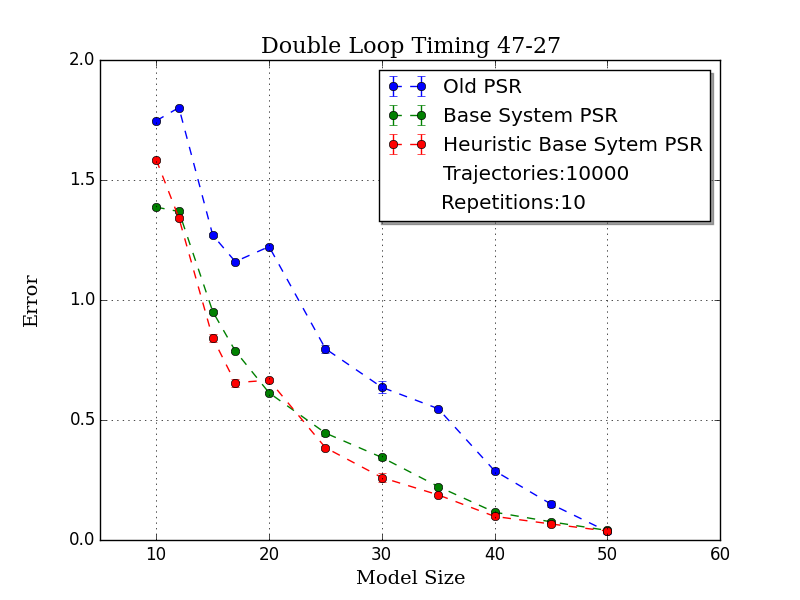
\includegraphics[width=60mm]{uCOREPICS/DoubleLoopTimingHeuristics47-27.png}
\caption{Double Loop Environment\label{overflow}}
\end{figure}

\begin{figure}[ht!]
\centering
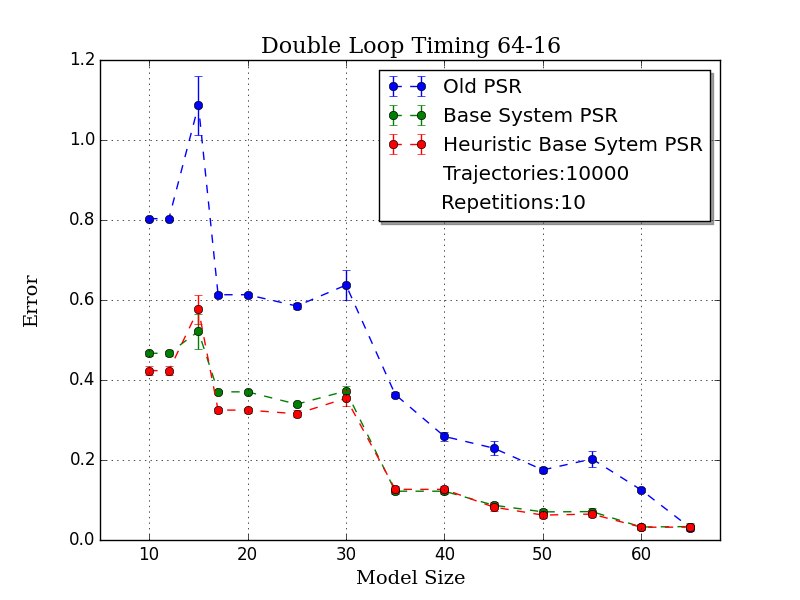
\includegraphics[width=60mm]{uCOREPICS/DoubleLoop64-16Heuristics.png}
\caption{Double Loop Environment\label{overflow}}
\end{figure}

\subsection{Pacman Timing}

We proceed to work with timing in a Pacman environment. The transition structure of this environment is shown in Figure 2. Edge weights vary from 1 to 3 and are stretched by a parmater we call the stretch factor which we initialize at 10. Again we use 10000 observation sequences per PSR and compute the average of 10 PSRs.

\begin{figure}[ht!]
\centering
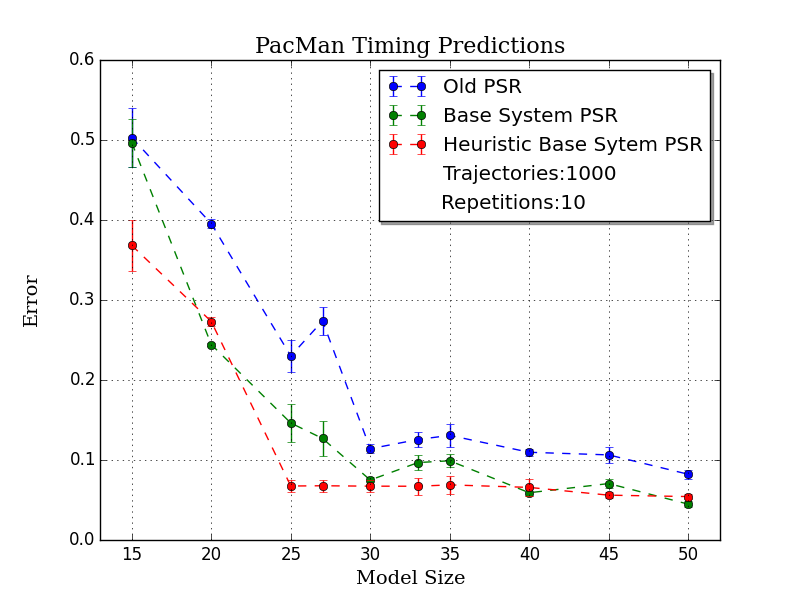
\includegraphics[width=60mm]{uCOREPICS/PacManTimingHeuristicsIncluded.png}
\caption{Double Loop Environment\label{overflow}}
\end{figure}

\subsection{Timing - Results}
As is demonstrated in figure 3, learning longer transitions provides a significant improvement over the standard for truncated models. The heuristic based approach performs slightly better than the powers of two method. For the double loop case the heuristic approach learns multiples of the loop lengths which results in partitions which use fewer operators. For Pacman, the operators that are learned are various multiples of the stretch factor, which once again shows that the greedy heuristic is effective. 

\subsection{Multiple Observations}

To test whether the Base System would translate to multiple observations we construct a double loop environment where one loop is green and the other is blue. The lengths of each loop are also varied. We fix the length of observations to be $loop1 + loop2 * 3$. To build empirical estimates of probabilities we set f(x)=prefix-occ(x)/num-strings-length>=x.

\subsection{Multiple Observations Results}

\begin{figure}[ht!]
\centering
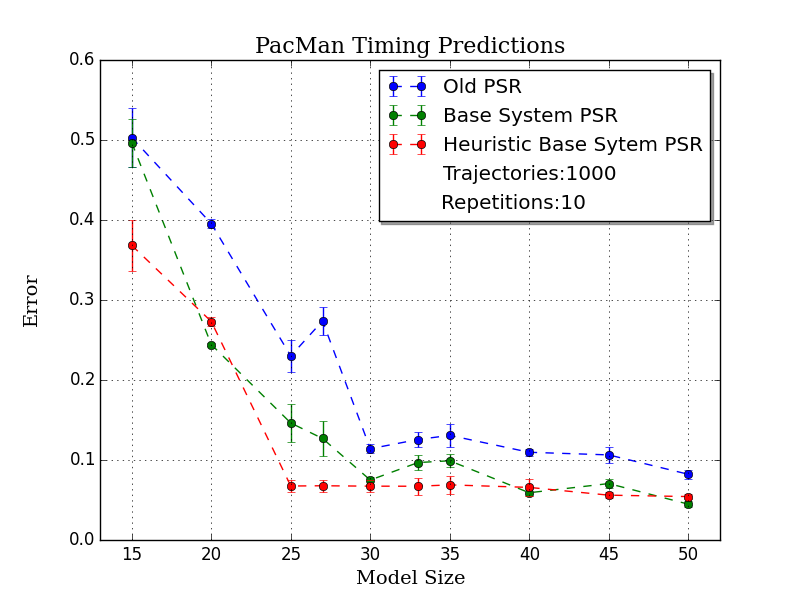
\includegraphics[width=60mm]{uCOREPICS/PacManTimingHeuristicsIncluded.png}
\caption{Double Loop Environment\label{overflow}}
\end{figure}


\section{Conclusion}

\section{Acknowledgments}
Funding and friends...

\bibliographystyle{aaai}
\bibliography{references}

\end{document}
